\begin{figure*}[hbtp]
  \centering
  \subfigure[Runtime in seconds (logarithmic scale) with \textit{Vite (Louvain)}, \textit{Grappolo (Louvain)}, \textit{NetworKit Louvain}, \textit{cuGraph Louvain}, and \textit{GVE-Louvain}]{
    \label{fig:louvain-compare--runtime}
    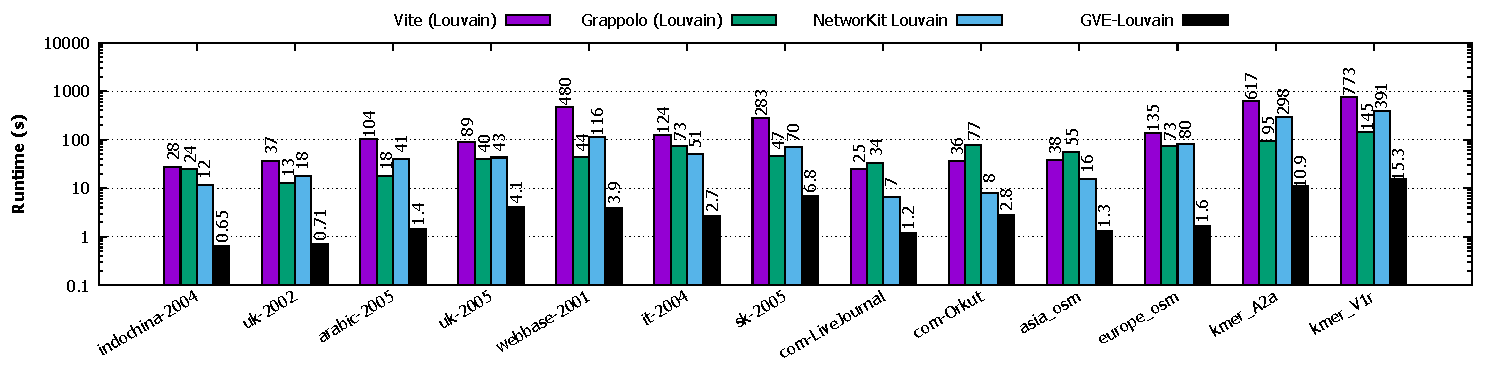
\includegraphics[width=0.98\linewidth]{out/louvain-runtime.pdf}
  } \\[-0ex]
  \subfigure[Speedup of \textit{GVE-Louvain} with respect to \textit{Vite (Louvain)}, \textit{Grappolo (Louvain)}, \textit{NetworKit Louvain}, and \textit{cuGraph Louvain}.]{
    \label{fig:louvain-compare--speedup}
    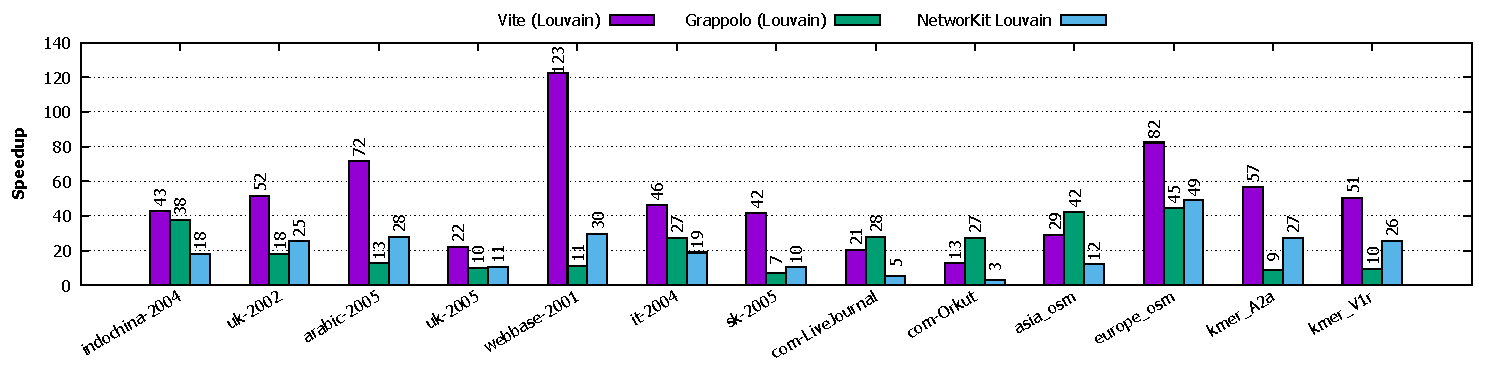
\includegraphics[width=0.98\linewidth]{out/louvain-speedup.pdf}
  } \\[-0ex]
  \subfigure[Modularity of communities obtained with \textit{Vite (Louvain)}, \textit{Grappolo (Louvain)}, \textit{NetworKit Louvain}, \textit{cuGraph Louvain}, and \textit{GVE-Louvain}.]{
    \label{fig:louvain-compare--modularity}
    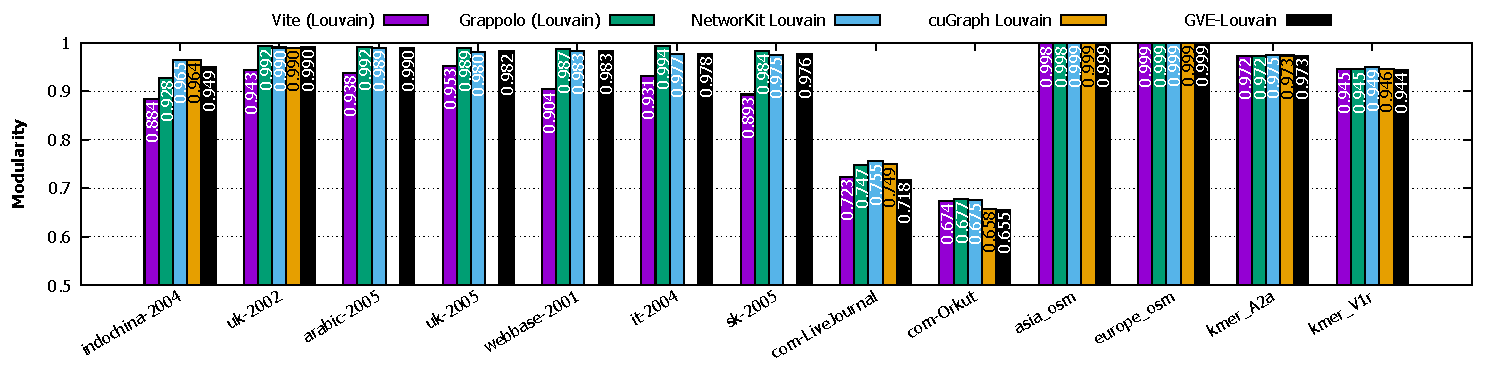
\includegraphics[width=0.98\linewidth]{out/louvain-modularity.pdf}
  } \\[-2ex]
  \caption{Runtime in seconds (logarithmic scale), speedup, and modularity of communities obtained with \textit{Vite (Louvain)}, \textit{Grappolo (Louvain)}, \textit{NetworKit Louvain}, \textit{cuGraph Louvain}, and \textit{GVE-Louvain} for each graph in the dataset.}
  \label{fig:louvain-compare}
\end{figure*}
